\documentclass[11pt,a4paper]{article}
\usepackage[english]{babel} %English hyphenation
\usepackage{graphicx} 
\usepackage{caption}
\usepackage{subcaption}
\usepackage{geometry}
\usepackage{sidecap}
\usepackage{gensymb}
\geometry{margin=25mm}
\usepackage[english]{babel}
\usepackage{hyperref}
\newcommand{\HRule}{\rule{\linewidth}{0.5mm}}

\begin{document}

\section*{Introduction}
Here I intend to document all my findings and reasoning on an experiment to create a prediction model for the NCAA lacrosse tournament. The goal is for this document to grow organically, each section being added as the results are done, with the thought process being written down throughout. 

\section*{Initial Data and Current State of the Field}
The only data we are starting with is the 2013-2017 regular seasons' game results. Explicitly a home-away team and how many goals each team scored. Further box results for each game can be found on the ncaa.org site, but will only be added later if/when needed. We also have access to a csv file that contains the NCAA tournament seedings and the results. 

Currently there are some analyses available for lacrosse games. Inside Lacrosse has a rudimentary predictor, and laxpower also contains a great deal of team statistics. lacrosseanalytics.com also contains some basic evaluation metrics such as strength of schedule and adjusted offensive efficiency. 

Lacrosse doesn't yet get the attention analysts have devoted to baseball or basketball prediction. Predictions are only a rough estimate about how likely a team is to win or score points, but they can also be seen as a tool to show which aspects of the game are keys to victory. 

\section*{Lacrosse Primer for the Uninitiated}
It is not unreasonable to assume (though unfortunate) that the reader isn't familiar with the game of lacrosse. Without going into too much depth, a few details are worth pointing out to be able to put the resulting analysis into context. 

\begin{itemize}
	\item Lacrosse is a semi-continuous game, played in four quarters. Semi-continous here means there are few breaks in action, save for referee interventions (timeouts, goals, penalties, injuries). Defensive to offensive transition can occur without a stoppage like in football. 
	\item Generally speaking, a goal leads to a faceoff (similar to ice hockey). Meaning a team that just scored can regain possession of the ball and go on another offensive attempt without the other team ever having control of the ball.
	\item NCAA lacrosse does not have ties. Overtime periods continue until a goal is scored and thus a winner emerges.
\end{itemize}

\section*{First Pass Through Data}
An initial exploration through the data shows the following:

\begin{tabular}{| c || c | c | c | c | c |}
	\hline
	year & home goals & away goals & games played & average home goals & average away goals\\ \hline \hline
	2013 & 5128 & 4692 & 477 & 10.75 & 9.84 \\ \hline
	2014 & 5478 & 4922 & 511 & 10.72 & 9.63 \\ \hline
	2015 & 5652 & 5052 & 522 & 10.83 & 9.68 \\ \hline
	2016 & 5688 & 5095 & 533 & 10.67 & 9.56 \\ \hline
	2017 & 5822 & 5325 & 537 & 10.84 & 9.92 \\ 
	\hline
\end{tabular}

\vspace{5mm}
This indicates home-field advantage of about one goal. Does this hold for all teams? Let's grab the top seeded team, middle ranked team, and lowest ranked team, according to laxpower, for each year to compare:

\begin{tabular}{| c || c | c | c | c |}
	\hline
	 & & games played & avg goals scored & avg goals allowed \\ 
	year & team & (home-away) & (home-away) & (home-away) \\\hline \hline
	2013 & Syracuse & 15-5 & 11.13-12.6 & 8.67-9.8 \\ \hline
	2013 & Army & 7-7 & 10.43-9.71 & 7.29-8.29 \\ \hline
	2013 & Wagner & 8-5 & 9.5-7.2 & 14.5-15.6 \\ \hline \hline
	2014 & Duke & 14-6 & 15.5-13.33 & 9.43-10.17 \\ \hline
	2014 & Saint Joseph's & 7-8 & 11.43-10.88 & 7.86-8.5 \\ \hline
	2014 & Wagner & 8-5 & 7-6.8 & 12.63-12 \\ \hline \hline
	2015 & Notre Dame & 10-5 & 12.9-14 & 9.4-9.2 \\ \hline
	2015 & Fairfield & 8-7 & 10-9.14 & 7.38-7.57 \\ \hline
	2015 & VMI\footnote{officially it was NJIT, but since they had just started their program and were fielding only freshmen, I discluded them to not skew the results} & 9-6 & 5.56-4.5 & 13.78-17.83 \\ \hline \hline
	2016 & Maryland & 12-8 & 12.58-10.13 & 8.66-7.88 \\ \hline
	2016 & Drexel & 6-9 & 9-8.89 & 8.33-10.22 \\ \hline
	2016 & VMI \footnote{As above, NJIT and Hampton were worse, but same reason} & 6-10 & 8.83-4.3 & 12-15.1 \\ \hline \hline
	2017 & Maryland & 11-8 & 12.91-11.88 & 8.36-9.38 \\ \hline
	2017 & Cornell & 6-7 & 13-10.57 & 11-15.57 \\ \hline
	2017 & NJIT \footnote{Hampton was still worse, but by now NJIT has been around enough to have some players} & 6-9 & 5.83-7.67 & 10.67-13.56 \\ \hline 
	\hline
\end{tabular}

\vspace{5mm}

With some exceptions, there does seem to be a trend of teams scoring more at home and giving up more goals when away. 

Now let's see the distribution of goals scored. Let's plot both home and away goals on the same plot.

\begin{figure}[htbp]
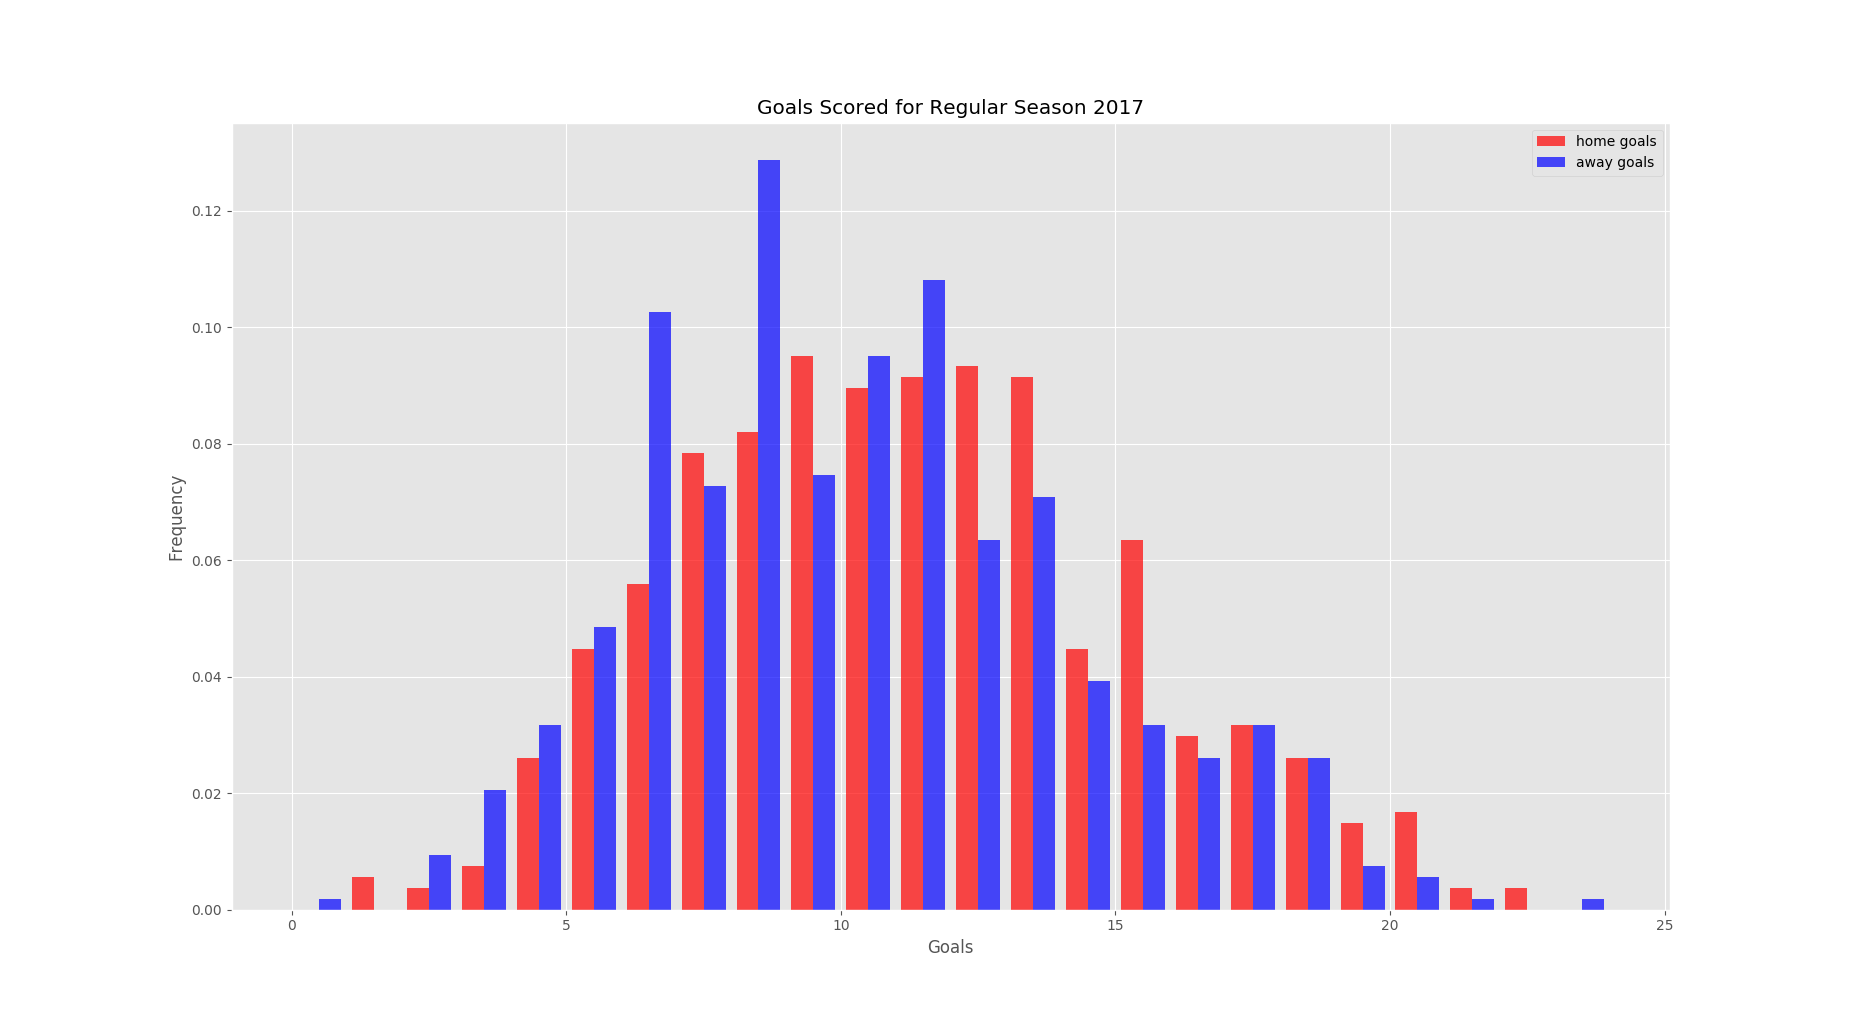
\includegraphics[width=\textwidth]{goals_2017.png}
\end{figure}

Looking at this plot, it seems to be a normal distribution. The results for years 2013-2016 look similar. Arguing a bit, one could say it looks a bit more like a skew normal distribution. With the limited sample size, we could probably fit a Poisson, Weibull or some other more distribution to the data. 

However, a much more interesting distribution to know would be an individual team's scoring distribution. Which any layman will tell you could be largely dependent on their opponent. This means we need more data for each team.

A clearer picture of the games can be obtained by plotting the goal differential for every home game. A negative goal differential would indicate a loss. 

\begin{figure}[htbp]
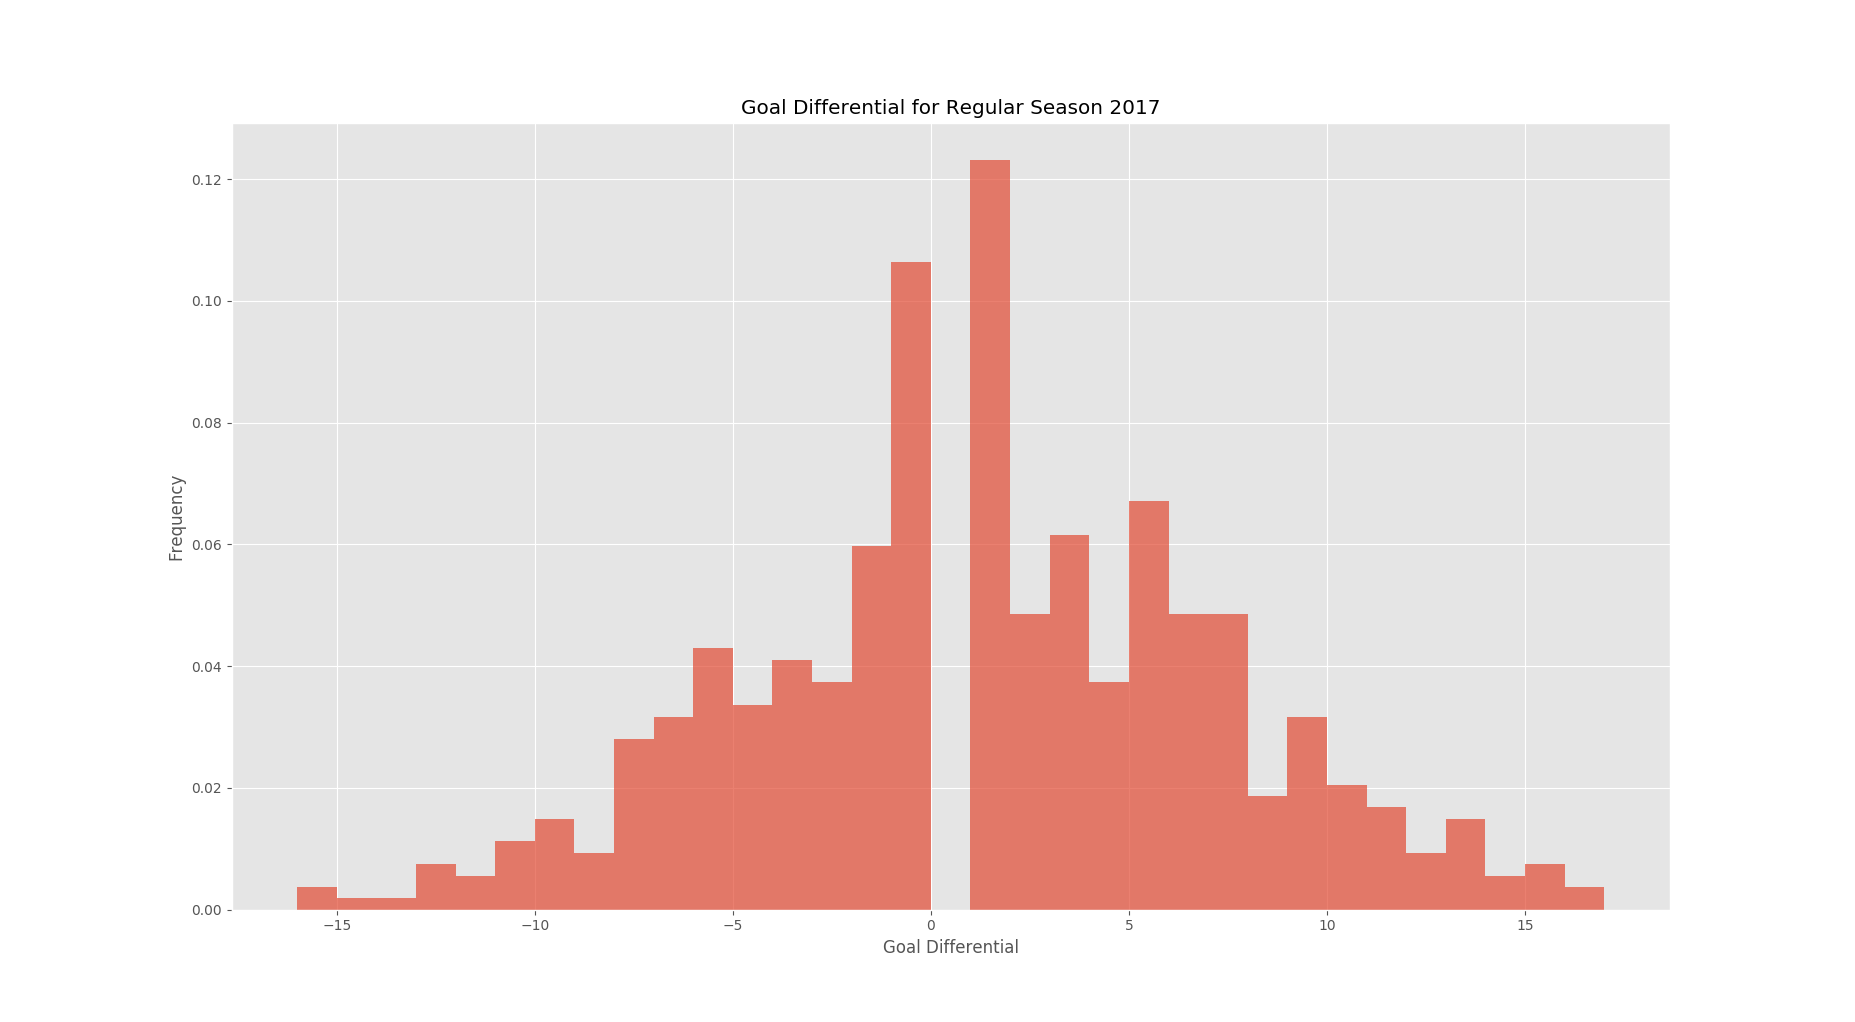
\includegraphics[width=\textwidth]{goal_diff_2017.png}
\end{figure}

Here we can see at a glance that about a quarter of all games were one-goal games. We can also note a distinct dropoff in frequency of games that had a larger than 7 goal differential. We can take the opportunity here to define a greater than 7 goal differential as a blow-out.

    \begin{figure*}[htbp]
        \centering
        \begin{subfigure}[b]{0.475\textwidth}
            \centering
            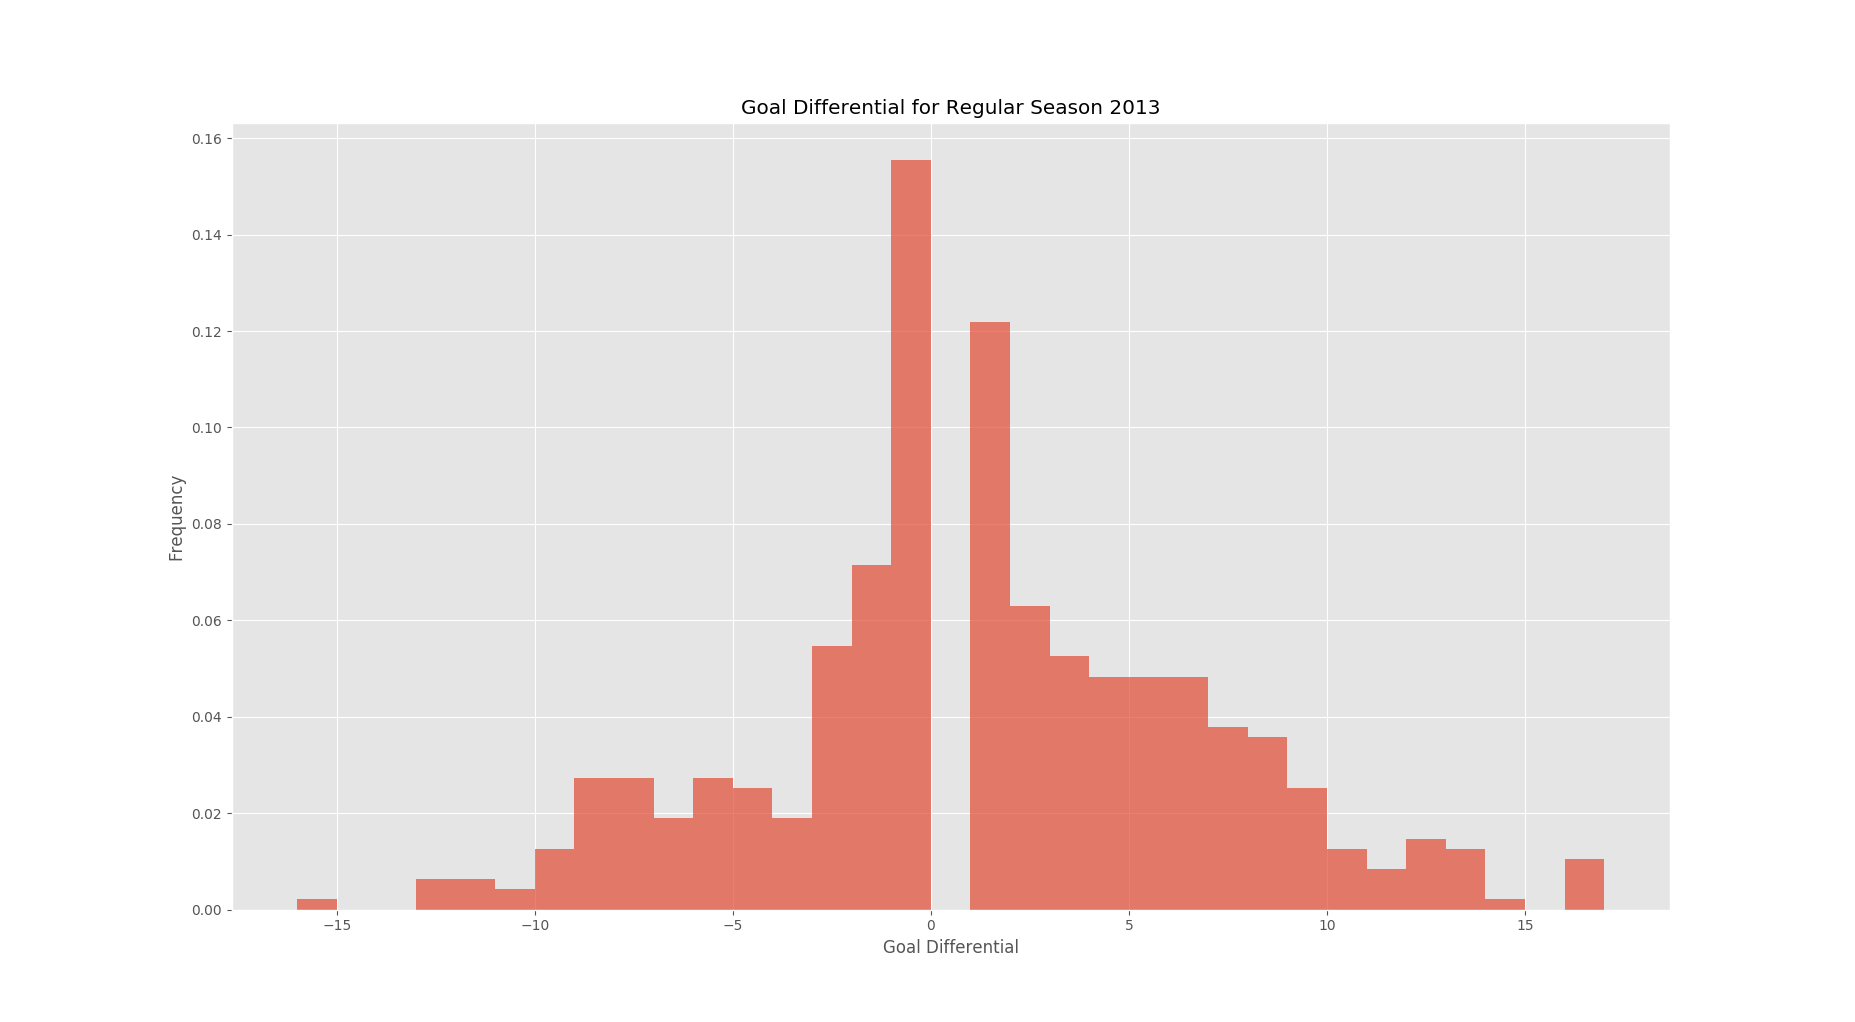
\includegraphics[width=\textwidth]{goal_diff_2013.png}
        \end{subfigure}
        \hfill
        \begin{subfigure}[b]{0.475\textwidth}  
            \centering 
            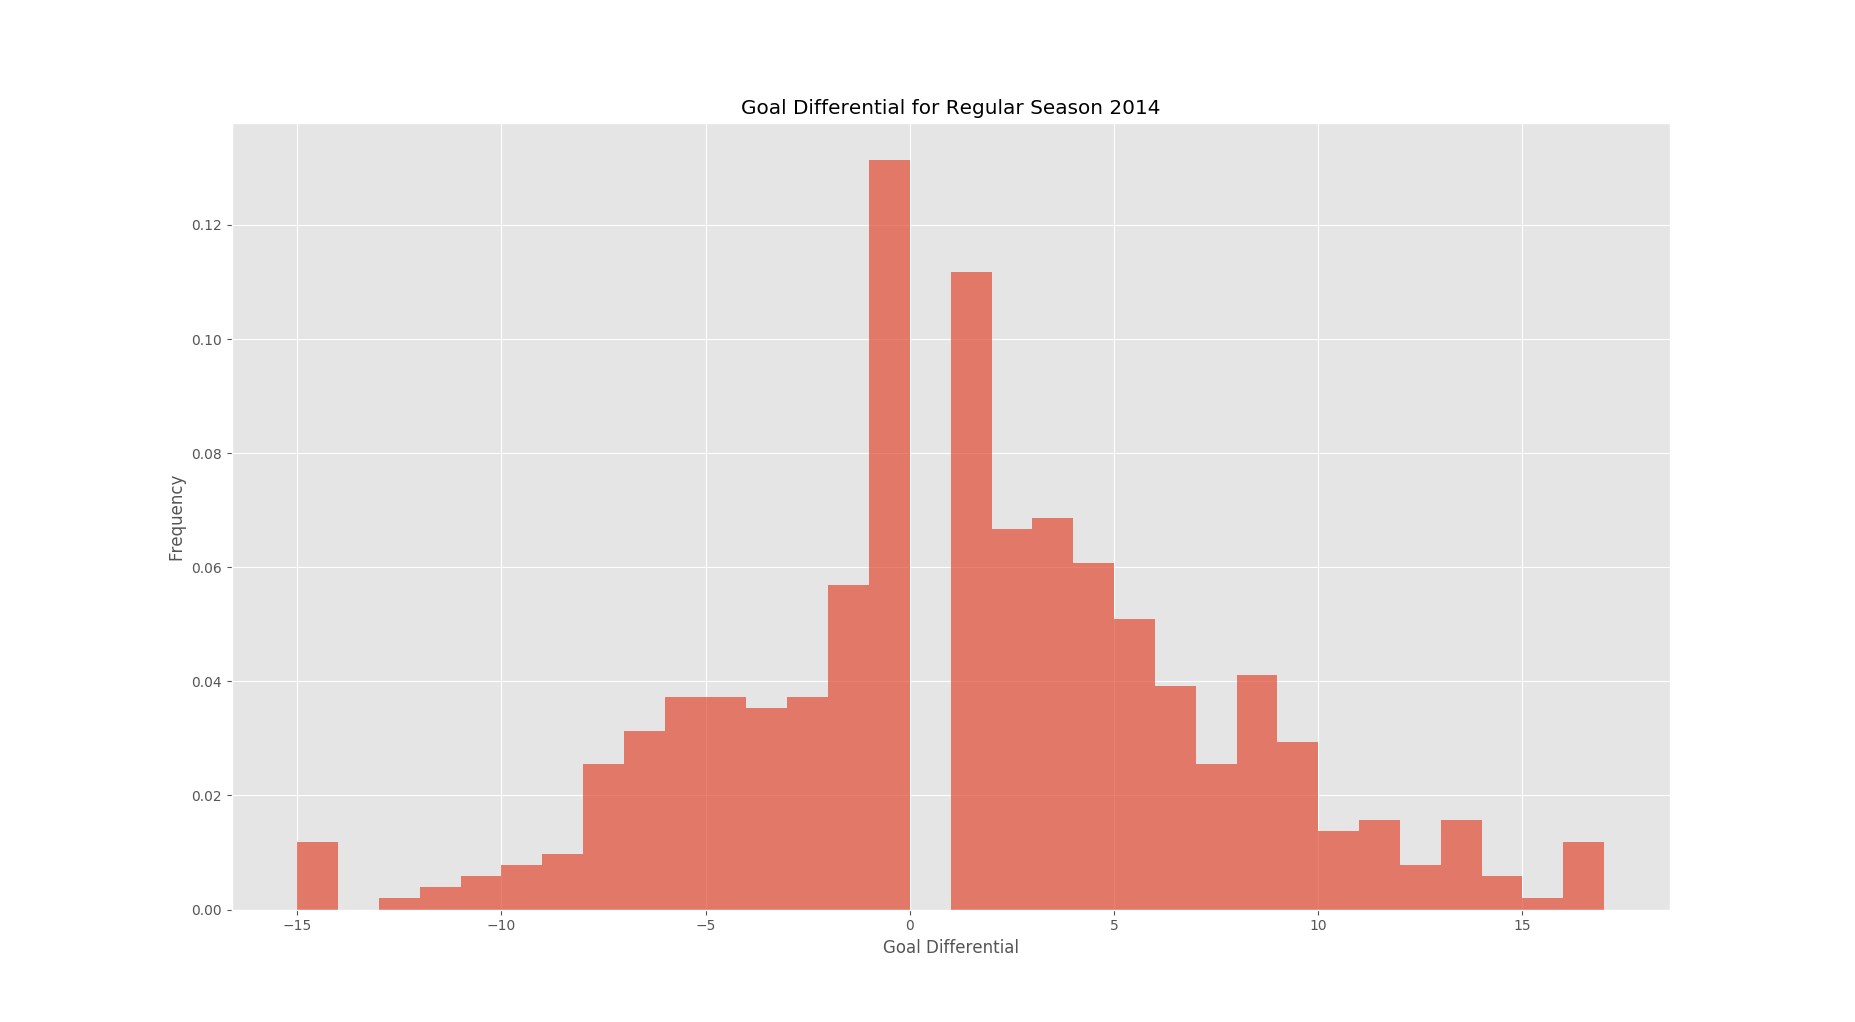
\includegraphics[width=\textwidth]{goal_diff_2014.png}
        \end{subfigure}
        \vskip\baselineskip
        \begin{subfigure}[b]{0.475\textwidth}   
            \centering 
            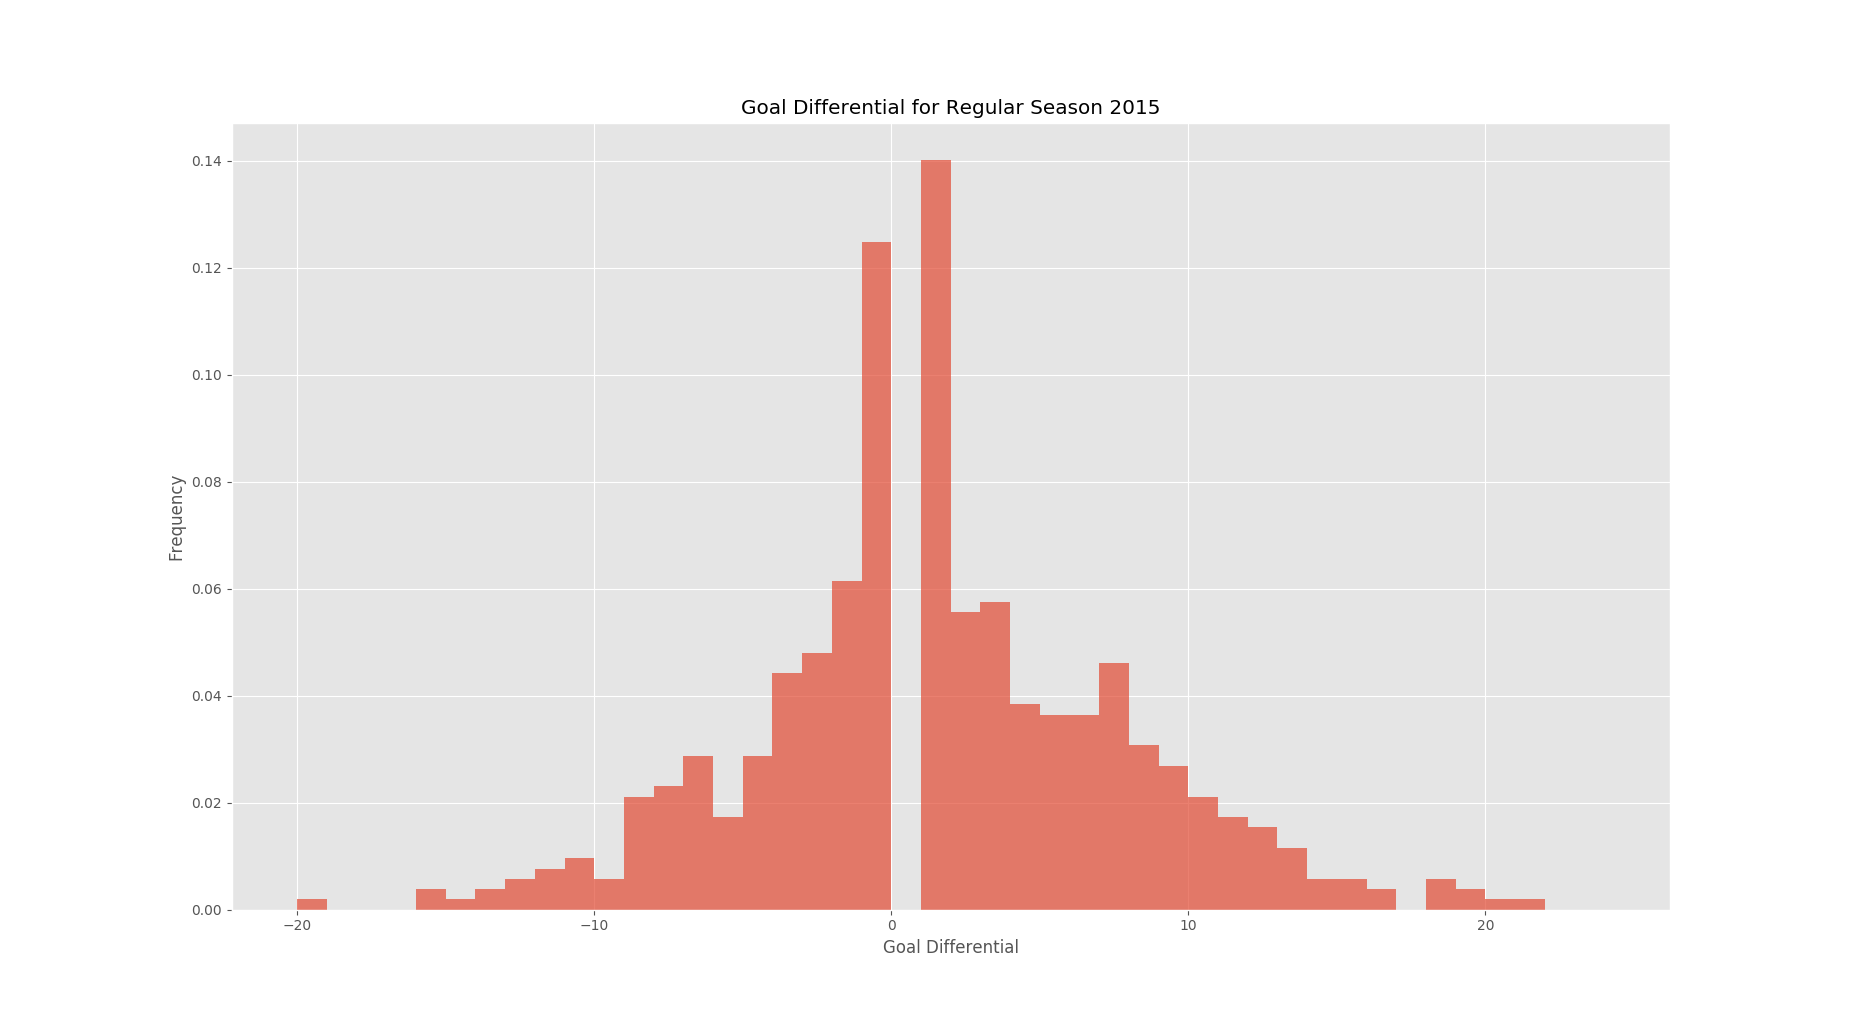
\includegraphics[width=\textwidth]{goal_diff_2015.png}
        \end{subfigure}
        \quad
        \begin{subfigure}[b]{0.475\textwidth}   
            \centering 
            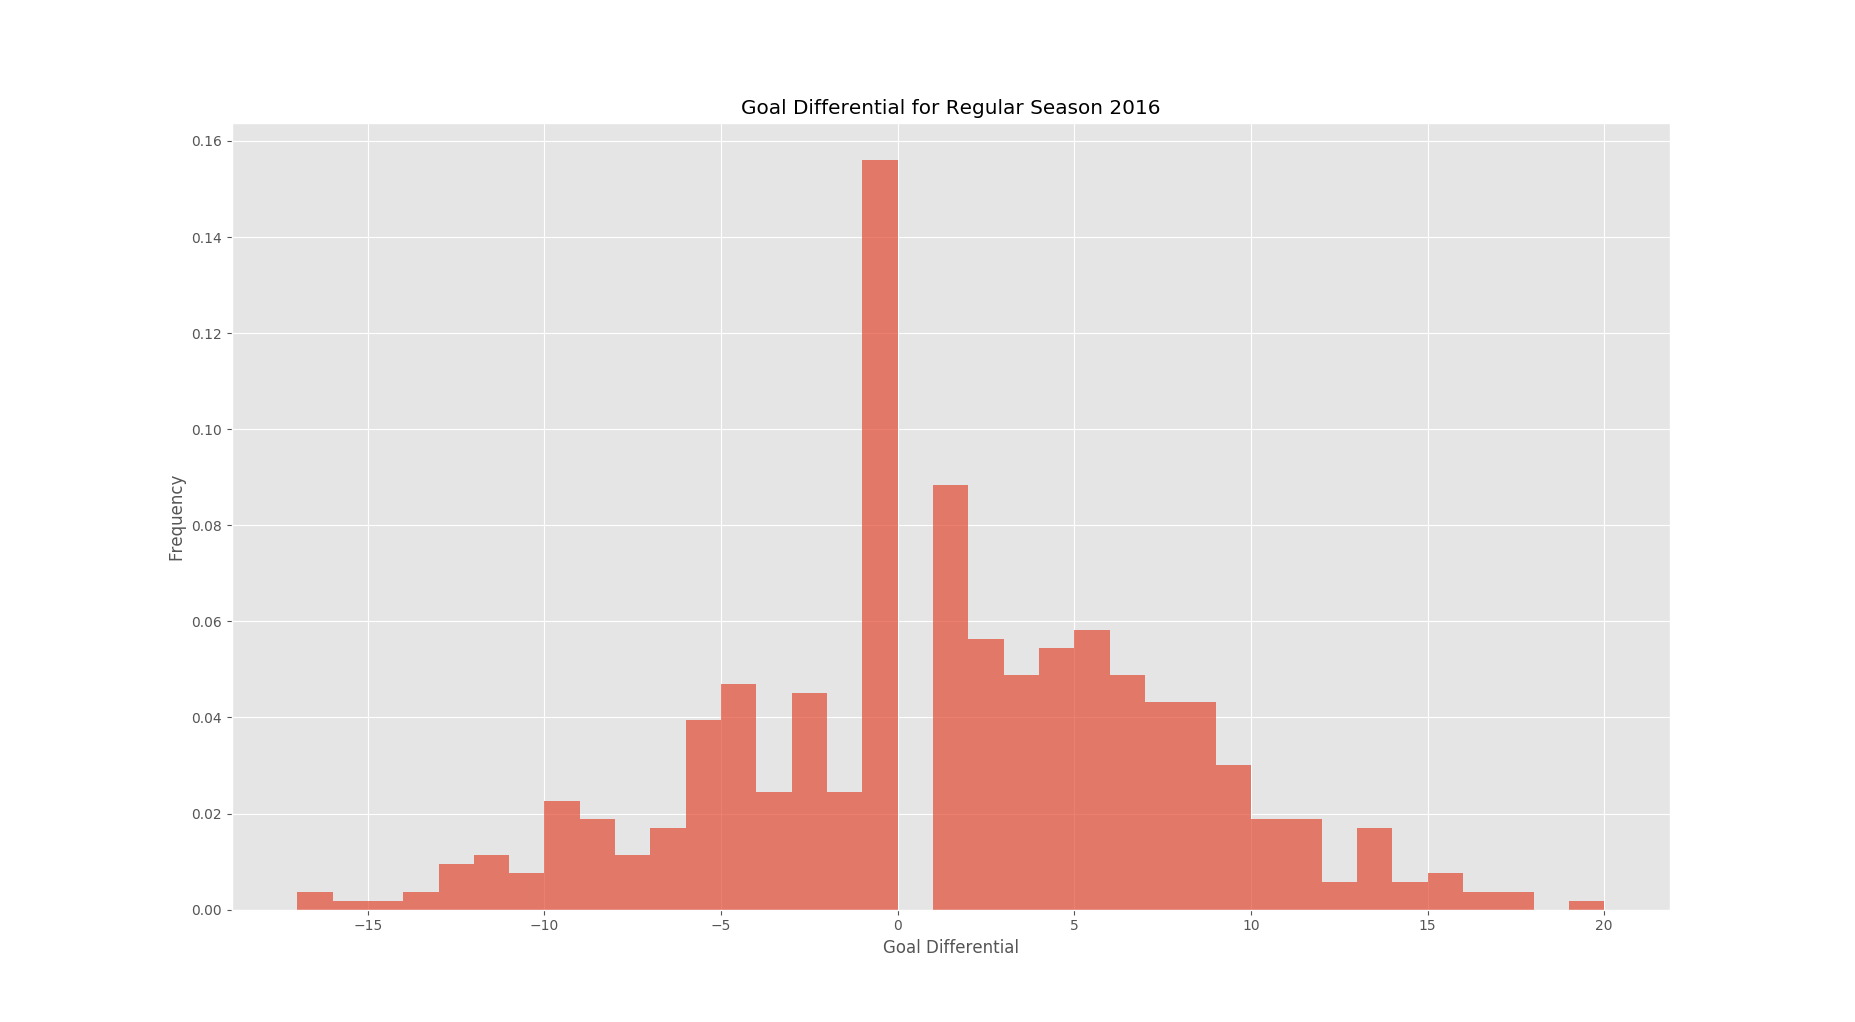
\includegraphics[width=\textwidth]{goal_diff_2016.png}
        \end{subfigure}
    \end{figure*}

Looking at the results from 2013-2016 as well, a similar trend starts to emerge. We note however that the home team frequently loses the one-goal games, especially in 2016 we note that if a game was close, the home team was more likely to lose the game than win it.

\section*{NCAA.org Data}
The NCAA hosts a website at ncaa.org where individual game statistics are available. In particular this allows us access to a finer granularity of data for each team. With data like goals, assists, groundballs, turnovers, faceoffs, penalties, saves and clears. Now each team can have their play evaluated off of a number of variables, with goals given up and goals scored being the values to predict. 

Another option is giving a team a single value score, or a multiple value. Analogous to a chess player's ELO rating, which we can give to the team as a whole, or to their respective units (offense, defense and face-offs). This could be more useful in allowing us to predict a match's results.

Accessing this data is relatively simple. The website uses GET parameters to get the individual team's statistics, so decyphering these parameters and their meaning will allow a scraper to go over the site and save the data locally.

Once the data is available locally, we can attempt a number of different methods to develop our rating and evaluate the matchups. 

\section*{Initial Thoughts For Matchup Predictor}
Having read how a number of the NCAA March Madness predictors work, it seems like adding a few data columns to the aggregated data will help us combine relevant data without having to pass the entire dataset through the model. 
Three different approaches present themselves for evaluation 
\subsection*{Autoencoder} 
Using an autoencoder we could throw the raw data into the autoencoder and allow it to spit out as many latent variables as we desire (one, three, ten, etc). Then we could connect this encoder to an evaluation function, which takes the output of the encoder for two teams playing one another and evaluates the result, backpropagating any errors to have the network learn. 
Since this is a neural network architecture, we can later decouple the various stages and have the autoencoder give us team ratings and predict future matchup success.

\subsection*{Team Probability Distributions}
Using the data, we could create a probability distribution of each team's results. Allowing for some weighting with the other team's Strength of Schedule (SOS, a variable we can calculate), the result of the game could be the weighted average of the results. This has the advantage of being simple to calculate, and we could use a Monte Carlo simulation (a fancy way of saying running it a lot of times) to generate an outcome probability.

\subsection*{Deep Learning}
As seems to be all the rage these days, we could create a large and deep network, throw each team's statistics into it and let the network figure it all out. With just over 2500 games presently available (we could probably get a few more seasons worth of data), there is some doubt if we have enough data to make a truly deep learning network converge on a satisfactory solution.

\subsection*{Other Regression Methods}
There are other regression methods that are available and possibly appropriate for these methods. In theory adding a naive bayes classifier, a support vector machine, and a random forest classifier, we could then take the results of all these models and stack them together to give a prediction. We may explore these options if the first two (or three, let's be honest, we could probably get away with a simple MLP for that).

\end{document}